\documentclass[]{article}
\usepackage{amsmath}
 \usepackage{graphicx}
%opening
\title{Microstate and Macrostate in Symbolic Dynamics of Chaotic Motion}
\author{Ilya Shesterikov}

\begin{document}

\maketitle


\begin{abstract}
The notions of microstate and macrostate, fundamental to statistical mechanics, are reformulated within the framework of symbolic dynamics for chaotic systems. Using a simple coin-toss model as a pedagogical starting point, we recall that the probability of a macrostate is determined by its multiplicity—the number of microstates realizing it—leading naturally to the principle of maximal probability and entropy. This concept is then extended to the fully chaotic Logistic map at ( r = 4 ). By encoding trajectories via a generating binary partition, we establish two complementary microstate–macrostate perspectives. In the first, phase-space points serve as microstates and finite symbolic sequences as macrostates; the multiplicity of a symbolic sequence is shown to be proportional to the size of the corresponding cluster of initial conditions and inversely proportional to the invariant probability density. In the inverted perspective, symbolic sequences are treated as microstates while finite phase-space intervals define macrostates, whose multiplicity directly reflects the local density of distinct symbolic encodings and is proportional to the invariant density. This dual formulation reveals a robust correspondence between invariant probability measure and informational density in symbolic space. Finally, exploiting the conjugacy of the Logistic map to the Bernoulli shift, we demonstrate that the non-uniform invariant density precisely guarantees equiprobability of all admissible symbolic sequences of fixed length. The results provide a transparent statistical-mechanical interpretation of symbolic dynamics and clarify the informational origin of invariant measures in fully chaotic systems.
\end{abstract}

\section{Introduction: Microstate and Macrostate in Chaotic Systems}



The concepts of \textbf{Microstate} and \textbf{Macrostate} are fundamental to the understanding of statistical mechanics.  
To illustrate these ideas, we consider the simple model of a coin-toss system. We examine $N=4$ identical coins, each of which is tossed once. Each coin can land in one of two possible states: Heads (H) or Tails (T). The total number of possible distinct outcomes or combinations is
\[
2^N = 2^4 = 16.
\]

A \textbf{Microstate} is a specific and detailed state of the system. It describes the state of each individual component.

For our coin system, a microstate corresponds to a specific outcome (heads or tails) for each individual coin.  
All possible microstates of the coin system are:

HHHH, HHHT, HHTH, HTHH, THHH, HHTT, HTHT, HTTH, THHT, THTH, TTHH, HTTT, THTT, TTHT, TTTH, TTTT.

Thus, all 16 distinct sequences of outcomes are microstates. Since each of these sequences is equally likely, the probability of each microstate is given by

\begin{equation}\label{key}
	p_i = \dfrac{1}{2^N} = \dfrac{1}{16}.
\end{equation}

The concept of a \textbf{macrostate} is a broad and coarse-grained description of the system, usually defined by a small set of macroscopic properties.

For the coin system, the macrostate can be defined by the total number of heads ($N_H$), ignoring the exact position of each coin.

Each macrostate can be realized by a different number of microstates. This number is called the \textbf{multiplicity} ($\Omega$).

\textbf{Realizations of the Macrostates}

The possible macrostates for $N=4$ coins, defined by the number of heads, are:
\begin{itemize}
	\item 0 Heads: TTTT ($\Omega = 1$ microstate)
	\item 1 Head:  HTTT, THTT, TTHT, TTTH ($\Omega = 4$ microstates)
	\item 2 Heads: HHTT, HTHT, HTTH, THHT, THTH, TTHH ($\Omega = 6$ microstates)
	\item 3 Heads: HHHT, HHTH, HTHH, THHH ($\Omega = 4$ microstates)
	\item 4 Heads: HHHH ($\Omega = 1$ microstate)
\end{itemize}

The \textbf{probability of a macrostate} is determined by its multiplicity, i.e.\ the number of microstates associated with it.
The probability $P(N_H)$ of a macrostate with $N_H$ heads is given by
\[
P(N_H) = \frac{\Omega(N_H)}{\text{total number of microstates}} = \frac{\Omega(N_H)}{16}.
\]

\begin{center}
	\begin{tabular}{|ccc|}
		\hline
		\textbf{Macrostate ($\mathbf{N_H}$)} & \textbf{Multiplicity ($\mathbf{\Omega}$)} & \textbf{Probability ($\mathbf{\Omega/16}$)} \\
		\hline
		0 Heads & 1 & $1/16$ \\
		\hline
		1 Head & 4 & $4/16 = 1/4$ \\
		\hline
		2 Heads & 6 & $6/16 = 3/8$ \\
		\hline
		3 Heads & 4 & $4/16 = 1/4$ \\
		\hline
		4 Heads & 1 & $1/16$ \\
		\hline
	\end{tabular}
\end{center}

The macrostate with 2 heads is the most probable, since it has the highest number of realizations, namely 6 microstates. If we toss the coins many times, we are most likely to observe 2 heads and 2 tails.

This leads to the fundamental principle of statistical mechanics:

\begin{quotation}
	\textbf{The most probable macrostate is the macrostate that has the largest number of microstates.}
\end{quotation}

This illustrates that systems naturally evolve toward the macrostate with the greatest number of corresponding microstates.
This state is referred to as the state of maximum entropy (the most disordered state).


The fundamental concepts of microstate and macrostate, central to statistical mechanics, offer a valuable framework for interpreting the relationship between symbolic dynamics and probability density in chaotic systems. In the context of the fully chaotic Logistic map  and its symbolic encoding, we propose an extension of the traditional definitions that rigorously connects the system's fine-grained state (phase space points) and its coarse-grained description (symbolic sequences) to the concepts of the microstate and macrostate.

The Logistic map provides an ideal and straightforward paradigm for developing foundational insights into the study of chaotic phenomena.
This map is defined by the following recurrence relation:

\begin{equation}
	x_{n+1} = f_r(x_n) =  r x_n (1 - x_n)	
	\label{fig:logistic_map}
\end{equation}



The map defines a process of iteration, where the output of the function at step $n$ becomes the input for step $n+1$. The sequence of values generated, $\{x_0, x_1, x_2, \dots\}$, is called an \textit{\textbf{orbit}}.
State Variable ($x_n$) - This is the variable whose value evolves over time. Mathematically, it is a real number restricted to the unit interval $I = [0, 1]$. This restriction is necessary to ensure that the next value, $x_{n+1}$, also remains within $[0, 1]$ when the parameter $r$ is in its relevant range $[0, 4]$.
The function $f_r(x)$ is a quadratic polynomial, making the system nonlinear. This nonlinearity is the source of its complex dynamics.
Control parameter ($r$) is a positive real number, typically restricted to $r \in [0, 4]$.
It acts as the "tuning knob" that determines the dynamical properties of the entire system. For $r=4$ the map is fully chaotic.

To apply symbolic dynamics, the continuous state space (the interval \([0, 1]\)) is divided into a finite number of regions, and each region
is assigned a \textbf{unique symbol}. An orbit, which is a sequence of real numbers \( x_0, x_1, x_2, \ldots \), is then converted into a \textbf{symbolic sequence} by recording the symbol of the region the trajectory visits at each time step.

A partition is classified as a \textbf{generating partition} if the correspondence between the infinite symbolic sequence and the original orbit is \textbf{one-to-one}. This means that studying the symbolic sequence alone can reveal the essential topological and measure-theoretic properties of the chaotic dynamical system. For one-dimensional maps like the Logistic Map, the boundary points of the partition are determined by the critical points and their preimages under the map.

For the fully chaotic Logistic Map with \( r = 4 \) (i.e., \( x_{n+1} = 4x_n(1 - x_n) \)), the state space \( I = [0,1] \) has a single critical point (the maximum of the parabola) at \( x_c = 0.5 \). The simplest and most fundamental \textbf{generating partition} is the \textbf{binary partition} defined by this critical point:

\begin{itemize}
	\item \textbf{Region 0 (Symbol L or 0)}: \( I_0 = [0, 0.5) \)
	\item \textbf{Region 1 (Symbol R or 1)}: \( I_1 = [0.5, 1] \)
\end{itemize}

The critical point \( x_c = 0.5 \) is the \textit{partition boundary}.

The symbolic sequence \( S = s_0 s_1 s_2 \ldots \) corresponding to an orbit \( x_0, x_1, x_2, \ldots \) is constructed using the following rule:

\[
s_n =
\begin{cases}
	0 \text{ (or L)} & \text{if } x_n \in [0, 0.5) \\
	1 \text{ (or R)} & \text{if } x_n \in [0.5, 1]
\end{cases}
\]

For example, if a trajectory is \( x_0 = 0.2, x_1 = 0.64, x_2 = 0.92, x_3 = 0.29, \ldots \), its symbolic sequence would be \( 0, 1, 1, 0, \ldots \).

Thus, if we take a sequence of 12 iterations, then to each initial point and its trajectory one can associate a certain sequence of symbols. For example, the trajectory of the initial point ($x_0 = 0.2$) can be encoded by the symbolic sequence  $[0,1,1,0,1,0,1,1,1,0,1,0]$. 

\begin{figure}[htbp]
	\centerline{\includegraphics[width=0.5\linewidth]{symbol_sequence.png}}
	\caption{The trajectory of any initial point $x_0$ in the phase space (x) can be mapped to a sequence of symbols consisting of 0s and 1s.}
	\label{fig:symbol_sequence}
\end{figure}

In other words, any initial point in the phase space can be mapped to a sequence of symbols consisting of 0s and 1s, as shown on the figure \ref{fig:symbol_sequence}.
Suppose that each initial point undergoes (N = 12) iterations in the course of its evolution. That is, we have 12 “cells” available to encode all possible trajectories.


\section{\textbf{Redefining the Microstate and Macrostate in Symbolic Dynamics of Chaotic Motion}}


In the following, we investigate the intrinsic relationship between the invariant probability measure of a dynamical system and the evolution of its associated symbolic sequences.
For the analysis of the Logistic Map on the continuous phase space ($I=[0,1]$), we employ two complementary approaches that provide microscopic and macroscopic descriptions of the dynamics from two mutually inverted viewpoints. The fully chaotic system of the Logistic Map possesses a unique, absolutely continuous invariant measure $\mu$, with a density function given by:
$$\rho(x) = \frac{d\mu}{dx} = \frac{1}{\pi \sqrt{x(1-x)}}, \quad x \in (0, 1)$$
This density dictates the long-term distribution of iterates $x_n$ within the phase space $X$. The non-uniform nature of $\rho(x)$—which approaches infinity at the boundaries $x=0$ and $x=1$ and is minimum at the critical point $x=0.5$—is a consequence of the map's quadratic shape. The orbits spend relatively more time near the boundaries than near the center.



In general, the understanding and interpretation of the probability measure depends on what we understand under the elementary information unit or an elementary microstate. Microstates are these elementary and equally probable system states which the system goes through in its evolutionary process. Which states are treated as equiprobable depends on the chosen analysis framework. In the one case, as an equiprobable microstate, one can choose the elementary small discretization of the phase space $X$, which will be initial points for the determination of the symbol sequences. For every sequence of symbols, there will be a corresponding number of elementary cells, $x_j$, which defines the probability of the given symbol sequence, or the given macrostate.

This logic can, however, be considered from another standpoint. 
In this way, an elementary symbol sequence can be chosen as an elementary and equally probable microstate. 
In turn, the macrostates can be defined as an elementary discretization of the phase space into small intervals $\Delta x_j$ which are, 
however, still large enough that each interval $\Delta x_j$ contains a number of symbol sequences S. 
Then the probability of a given $\Delta x_j$  will be determined by the number of the sequences falling in this interval.





\subsection{ Symbolic Sequences as Macrostates}

\textbf{In the first perspective}, the phase space $X$ of the Logistic map is uniformly discretized into a large number of contiguous subintervals, $\Delta x$, yielding an ensemble of \textbf{equidistant and equally probable initial points}. So, we define a \textbf{Microstate} as one of the individual, equidistant initial points $x_i$ from the discretized phase space ensemble. Each such point represents a unique, fine-grained specification of the system's initial condition. The total number of such points (Microstates) is proportional to $1/\Delta x$.
A \textbf{Macrostate} is defined by a specific, finite-length \textbf{symbolic sequence} $S$ (e.g., $S = [s_0s_1s_2...s_{K-1}]$ where $K$ is the length of the sequence). 
This is illustrated in the Figure \ref{fig:symbol_sequence_linspace}.


\begin{figure}[h!]
	\centering
	\includegraphics[width=0.5\linewidth]{symbol_sequence_linspace.png}
	\caption{Illustration of partitioning the phase space $x \in [0, 1]$ into equally sized intervals. 
		Each point $x_i$ of an interval designates a certain Microstate. Several distinct nearby points in the phase space, such as the one labeled $x_i$ and its neighbors, may correspond to the same symbolic sequence (e.g., $[0,1,1,0,1,0,0,1,1,0,1,0]$), forming a small cluster of nearby points that are indistinguishable due to the finite symbol resolution. This cluster and the corresponding symbol sequence designate a certain Macrostate.}
	\label{fig:symbol_sequence_linspace}
\end{figure}


Since symbolic dynamics involves the encoding of trajectories, a single symbolic sequence is a \textbf{coarse-grained description} of the system's evolution. Multiple distinct, nearby initial points (Microstates) may correspond to the exact same symbolic sequence or the same Macrostate. The critical point in this concepts is the realization that a single Macrostate (symbolic sequence) is not unique to a single Microstate (initial point) but corresponds to an \textbf{entire cluster} of nearby initial points in the phase space. 
This cluster represents the set of indistinguishable points, given the finite resolution of the symbolic encoding.

The Multiplicity ($\Omega$) of a Macrostate is the number of Microstates that realize that particular Macrostate. In the context of the symbolic dynamics framework, the Multiplicity of a symbolic sequence $S$ is precisely the Cluster Size, denoted as $N(x)$. The cluster size $N(x)$ measures how many of the initial $\Delta x$ intervals map to the same symbolic sequence $S$.

The fundamental principle of statistical mechanics—that the probability of a Macrostate is proportional to its Multiplicity—can now be directly applied:

$$P(S) \propto \Omega(S) = N(x) $$

where $P(S)$ is the probability of observing the specific symbolic sequence $S$, and $N(x)$ is the size of the cluster in the phase space that encodes $S$. 
This probability $P(S)$ is effectively the measure (length) of the phase space interval corresponding to the sequence $S$.
Consequently, a symbolic sequence that is observed more frequently must, by definition, be encoded by a larger cluster of initial points.
A large cluster size $N(x)$ means many initial points (Microstates) are required to generate the same sequence $S$ (Macrostate).
This Macrostate is thus more probable but, simultaneously, less informative.
This phenomenon occurs in regions of the phase space where the dynamics expand slowly, making nearby points remain "close" and indistinguishable for a longer time under finite symbolic resolution. In opposite, a small cluster size $N(x)$ means the sequence $S$ is rare, but highly specific; it has a high resolution and is thus highly informative. This typically occurs in regions where the map stretches the phase space quickly, pushing nearby initial points apart rapidly.


The cluster size $N(x)$ (Multiplicity) is inversely proportional to the local informativeness of the symbolic encoding. 
Thus, the inversion of the cluster size, $1/N(x)$, represents this local informativeness. 
Crucially, the earlier work established that this local informativeness, $1/N(x)$, exhibits the same functional dependence as the analytical invariant probability density, $\rho(x)$.

$$\rho(x) \propto \frac{1}{N(x)} $$

y combining equations (2) and (3), we arrive at a robust conclusion:

$$P(S) \propto N(x) \propto \frac{1}{\rho(x)} $$

This confirms that the probability of a Macrostate (symbolic sequence) is inversely proportional to the system's local invariant probability density $\rho(x)$.


\subsection{The Inverted Perspective: Phase Space Discretization as Macrostates}


Let us invert the relationship established in the previous Section and consider the uniform phase space discretization as the coarse-grained, or "macroscopic" definition, while the symbolic clusters represent the "microscopic" realizations.
This is illustrated in the Figure \ref{fig:symbol_sequence_inverted}.

\begin{figure}[h!]
	\centering
	\includegraphics[width=0.6\linewidth]{symbol_sequence_inverted.png}
	\caption{Inverted microstate–macrostate perspective. The phase space ($x \in [0,1]$) is uniformly discretized into finite intervals ($\Delta x_j$), which now define the macrostates. Each interval ($\Delta x_j$) contains multiple distinct symbolic sequences ($S_k$) of fixed length ($N$), which constitute the microstates. The multiplicity ($\Omega(\Delta x_j)$) is given by the number of unique symbolic sequences within the interval and represents the local informational density. Regions with larger ($\Omega(\Delta x_j)$) correspond to higher invariant probability density ($\rho(x)$).
	}
	\label{fig:symbol_sequence_inverted}
\end{figure}

We begin by establishing the new definitions based on the uniform discretization of the phase space $I=[0,1]$ into equal-measure contiguous subintervals, $\Delta x$.
A \textbf{Macrostate} $M_j$ is defined by a specific, finite subinterval $\Delta x_j$ of the phase space.
The length of subintervals $\Delta x_j$ is such that within each subinterval fall a number of symbol sequences.
A \textbf{Microstate} $\mu_k$ is defined by a specific, unique symbolic sequence $S_k$ of length $N$. 
Each unique sequence $S_k$ corresponds to a certain interval $\Delta x_j$ in the phase space. 
So, each macrostate corresponds to many symbol sequences or many microstates, as shown in the Figure \ref{fig:symbol_sequence_inverted}.

\textbf{Under this inversion, the core question becomes: How many Microstates (unique symbolic sequences) fall into a given Macrostate (a certain interval $\Delta x_j$)?}

Under this new perspective: The Multiplicity ($\Omega$) of a Macrostate $\Delta x_j$ is the number of distinct Microstates (unique symbolic sequences $S_k$)  contained within the interval $\Delta x_j$.
$$\Omega(\Delta x_j) = (\text{Number of unique symbolic sequences } S_k \text{ in } \Delta x_j)$$

Thus, the Multiplicity, $\Omega(\Delta x_j)$, represents the \textbf{local density of unique information units} within the Macrostate $\Delta x_j$.
Where $\Omega(\Delta x_j)$ is large, the uniform phase space interval $\Delta x_j$ is realized by a large number of distinct symbolic sequences (Microstates). 
According to the first key finding, this density of unique symbolic encodings is highest in regions where the invariant probability density $\rho(x)$ is highest.

$$\Omega(\Delta x_j) \propto \rho(x_j)$$
Where $\Omega(\Delta x_j)$ is small, the interval $\Delta x_j$ is encoded by only a few distinct sequences. This corresponds to regions where the invariant probability density $\rho(x)$ is low.

In this inverted perspective, the most probable Macrostate is the phase space interval $\Delta x_j$ that contains the largest number of unique symbolic Microstates. 
This result affirms the principle of statistical mechanics: 
The region of the phase space where the system is most likely to be found (high $\rho(x)$) is precisely the region of the highest informational density (highest Multiplicity $\Omega(\Delta x)$).

This framework provides a direct mechanism for how the phase space measure is "weighted" by the intrinsic information structure of the chaotic system. The symbolic encoding (Microstates) partitions the phase space such that regions with a higher density of these partitions correspond exactly to regions of high invariant probability. The time the system spends in the interval $\Delta x_j$ is determined by the integral of $\rho(x)$ over that interval:

$$P_{\text{time}}(\Delta x_j) = \int_{\Delta x_j} \rho(x) dx \approx \rho(x_j) \cdot \Delta x $$

\subsection{Invariant Density and Symbolic Dynamics of the Logistic Map}

The very methodology of measuring the invariant measure, as well as the meaning of this measure as the frequency with which points of the phase space are visited during their chaotic evolution, implies that the probability distribution in the second approach will be determined by the invariant measure. Indeed, if we consider an infinitely long trajectory in the phase space and divide this trajectory into many segments of equal length — say, with N = 12 values each — and encode each segment by a symbol sequence ( S ), then the regions of the phase space ( X ) that naturally contain a high density of points will accordingly also contain a higher density of the symbols ( S ), and vice versa. So the distribution density of different S within the space of X will be our invariant probability density.

The profound connection between the invariant probability density $\rho(x)$ of the fully chaotic Logistic Map and the uniformity of its generated symbol sequences stems from the underlying topological conjugacy of the system to the Bernoulli Shift map. 
The key to understanding the symbolic dynamics is the \textbf{conjugacy transformation}. 
The Logistic map $f(x)$ is topologically conjugate to the piecewise linear Tent Map $T(y)$:
$$T(y) = \begin{cases} 2y, & 0 \leq y \leq 1/2 \\ 2(1-y), & 1/2 < y \leq 1 \end{cases}$$
via the coordinate change $x = h(y) = \sin^2\left(\frac{\pi}{2} y\right)$. 
The Tent Map itself is metrically isomorphic to the Bernoulli Shift $B(z) = 2z \pmod 1$. The invariant density for both $T(y)$ and $B(z)$ is $\rho_{T/B}(y) = 1$, indicating a uniform distribution of iterates in their respective coordinate systems.


A finite symbol block of length $k$, $S^k = S_0 S_1 \ldots S_{k-1}$, corresponds to a specific sub-interval $\Delta_{S^k} \subset I$ of initial conditions $x_0$ such that the trajectory $x_0, x_1, \ldots, x_{k-1}$ follows the sequence of partitions specified by $S^k$. This interval $\Delta_{S^k}$ is found by taking the inverse image:
$$\Delta_{S^k} = \{x_0 \in I \, | \, x_i \in I_{S_i} \text{ for } i=0, \ldots, k-1\} = I_{S_0} \cap f^{-1}(I_{S_1}) \cap \cdots \cap f^{-(k-1)}(I_{S_{k-1}})$$

The probability of observing the symbol block $S^k$ is given by the invariant measure of the corresponding interval:
$$P(S^k) = \int_{\Delta_{S^k}} \rho(x) \, dx$$

The critical result is that, despite the non-uniform density $\rho(x)$ in the phase space, the probability of every admissible symbol block interval $\Delta_{S^k}$ of length $k$ is exactly the same. For the fully chaotic Logistic map, the symbolic dynamics are equivalent to the \textbf{full $2$-shift}, meaning all $2^k$ possible sequences $S^k$ are admissible and equally probable. This is where the specific analytical form of $\rho(x)$ plays its role: it ensures the \textbf{equipartition of the invariant measure} across the symbol space.

The measure of every $k$-block is found to be:
$$P(S^k) = \mu(\Delta_{S^k}) = \frac{1}{2^k}$$
This result confirms that, when viewed through the lens of symbolic dynamics, the Logistic Map at $a=4$ behaves exactly like an independent, identically distributed (IID) process where $P(0) = P(1) = 1/2$, akin to a fair coin toss.

In essence, the non-uniform density $\rho(x)$ in the phase space is the exact distribution required to compensate for the non-linear distortion of the map $f(x)$ on the interval lengths, ensuring that the invariant measure of all generated symbol sequence intervals is uniform. This maximal randomness, characterized by the symbolic equipartition, is quantified by the system's Kolmogorov-Sinai entropy being $\ln 2$, the maximum possible for a binary process. \textbf{The invariant density $\rho(x)$ is thus the density that makes the symbol sequence probability uniform. }

\end{document}